\section{Discussão}\label{sec:discussao}

Os quatro tratamentos formam um desenho $2\times 2$ (presença de allowlist $\times$ adulteração do \texttt{.ino}), resumido na Figura~\ref{fig:matriz-experimental}. O resultado que organiza a discussão é binário e reproduzível no lote de amostras: \emph{somente} o caminho com segurança e firmware adulterado é recusado (HTTP 403, zero transações). Nos outros três, a IOTA EVM Testnet aceita a chamada ao contrato \texttt{registrar} com HTTP 200 (Figura~\ref{fig:leituras-aceitas}). A cadeia, portanto, registra o que o \emph{relay} deixa passar; ela não inspeciona o firmware.

\begin{figure}[htbp]
\centering
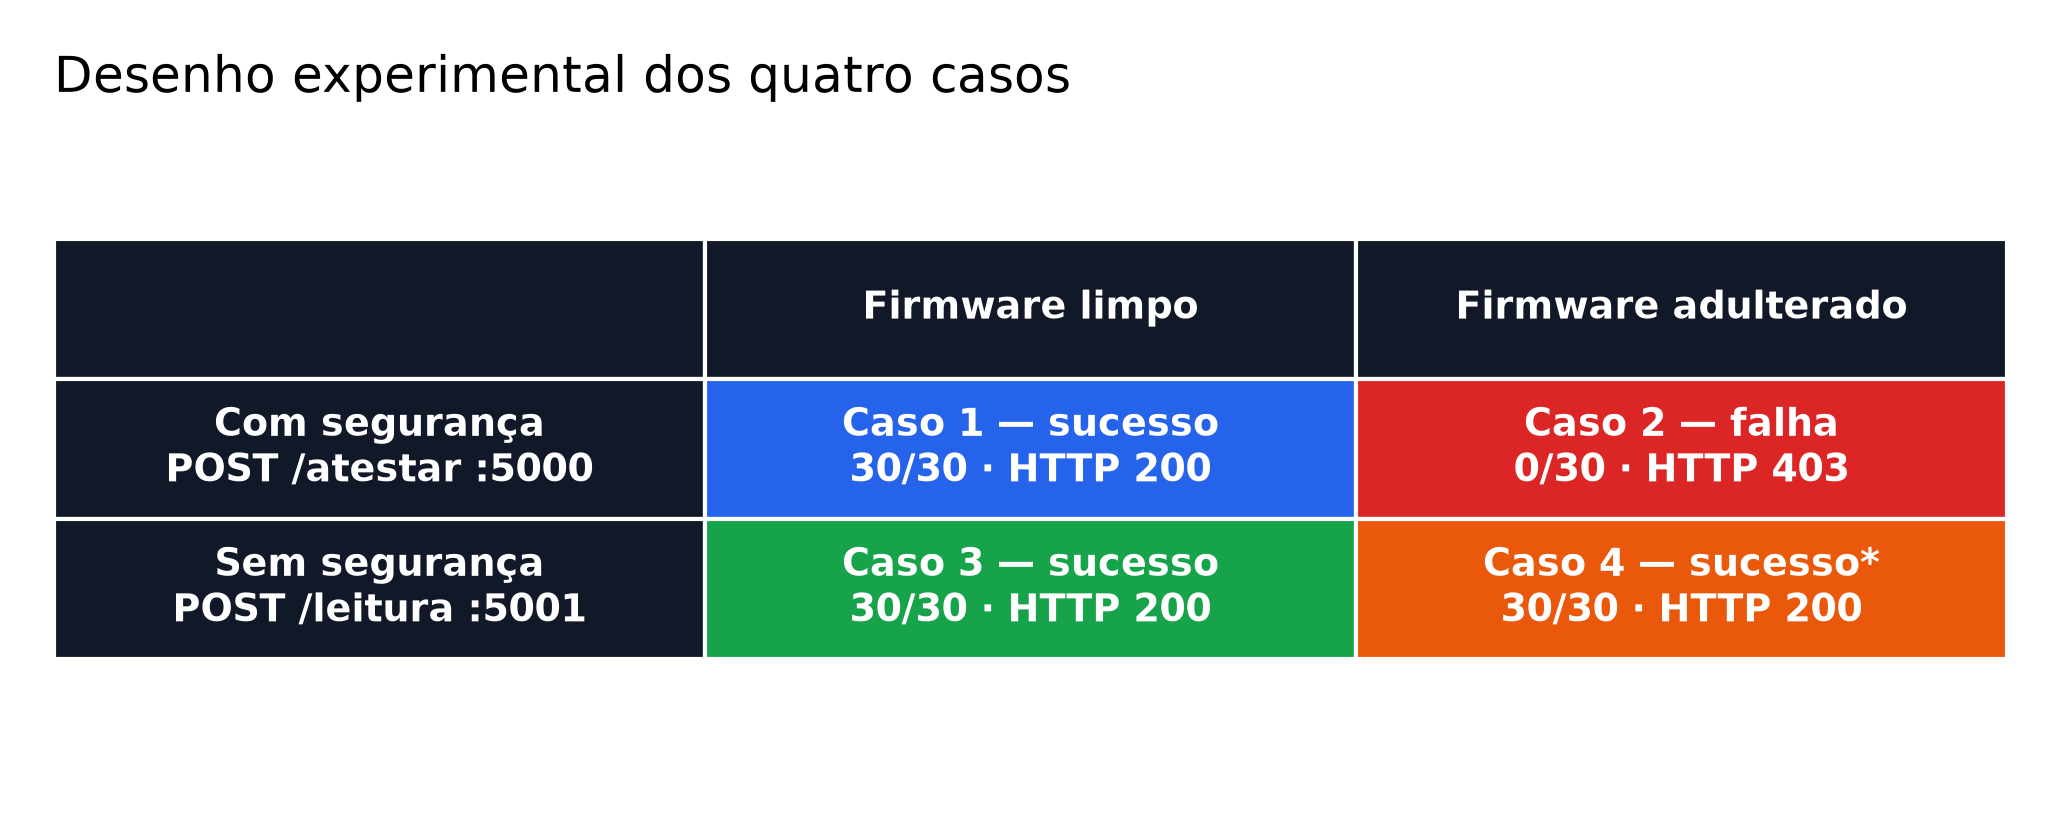
\includegraphics[width=0.92\textwidth]{figuras/matriz-experimental.png}
\caption{Desenho experimental dos quatro tratamentos (allowlist $\times$ adulteração do \texttt{.ino}).}
\label{fig:matriz-experimental}
\end{figure}

\begin{figure}[htbp]
\centering
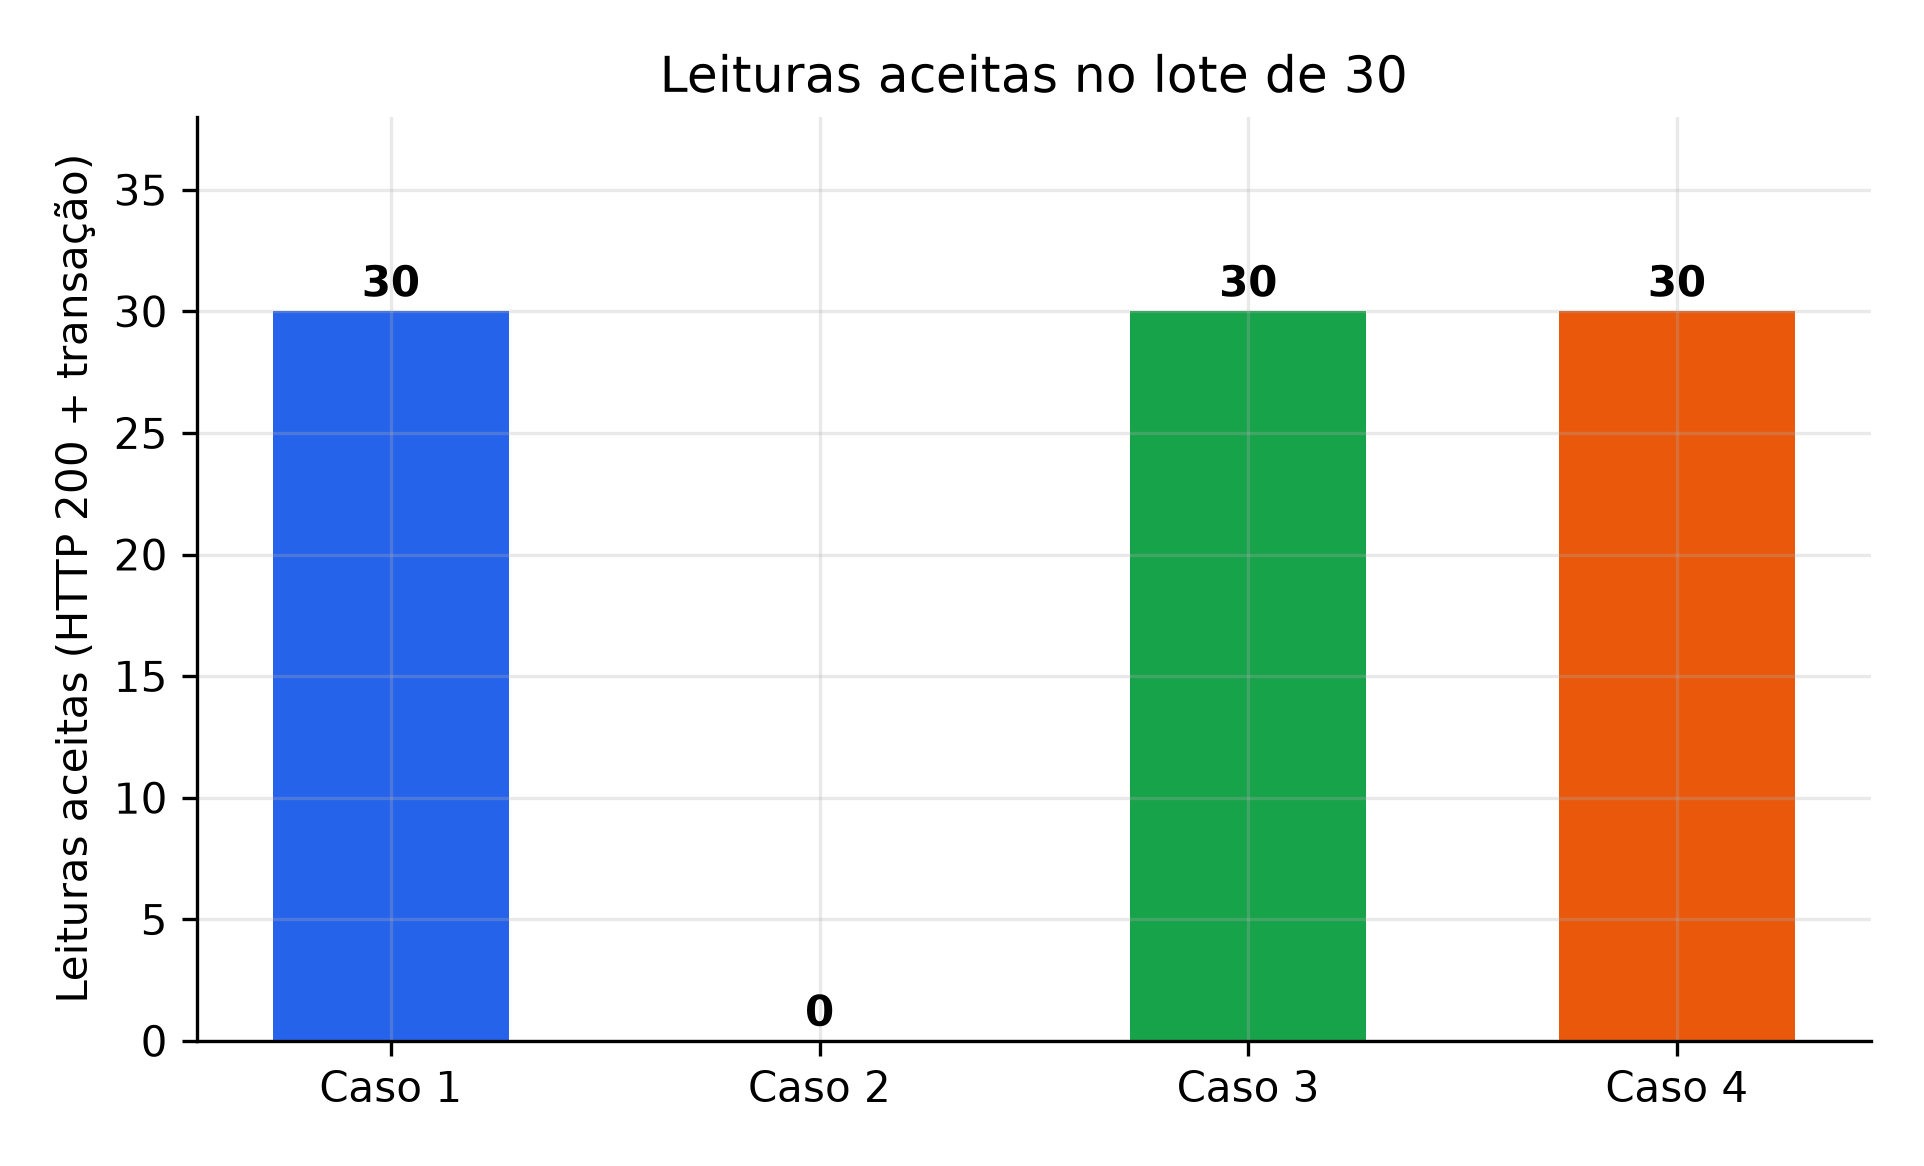
\includegraphics[width=0.82\textwidth]{figuras/leituras-aceitas.png}
\caption{Leituras aceitas em cada tratamento. Apenas o caminho com segurança e firmware adulterado não gera transação.}
\label{fig:leituras-aceitas}
\end{figure}

A comparação com versus sem adulteração, \emph{com} a allowlist ligada, mostra que o filtro de hash cumpre o papel de atestação neste protótipo. O hash enrolado é aceito nas leituras do Caso~1; o hash apresentado após o \texttt{Serial.println} no \texttt{.ino} é rejeitado nas leituras do Caso~2, \emph{antes} de haver custo de gás. A mesma adulteração, \emph{sem} allowlist (Caso~4), grava na cadeia de forma indistinguível do firmware limpo (Caso~3): mesmo gás médio, mesmo custo por transação e no lote, e a mesma taxa de sucesso. Sem o enrolamento no relay, a publicação on-chain não denuncia o código alterado.

O custo não é o termo que separa ``seguro'' de ``inseguro'' neste lote, como se vê na Figura~\ref{fig:custo}. Nos três casos com transação o gás foi \emph{idêntico em todas as amostras} ($s=0$): cabe no fato de os dois caminhos chamarem o mesmo contrato \texttt{registrar}, e não num ``preço da atestação'' isolado. O Caso~2 custa zero precisamente porque a política de hash aborta o fluxo. Interpretar $s=0$ no custo como precisão estatística seria um erro: o desvio nulo só diz que a máquina virtual repetiu o mesmo opcode path.

\begin{figure}[htbp]
\centering
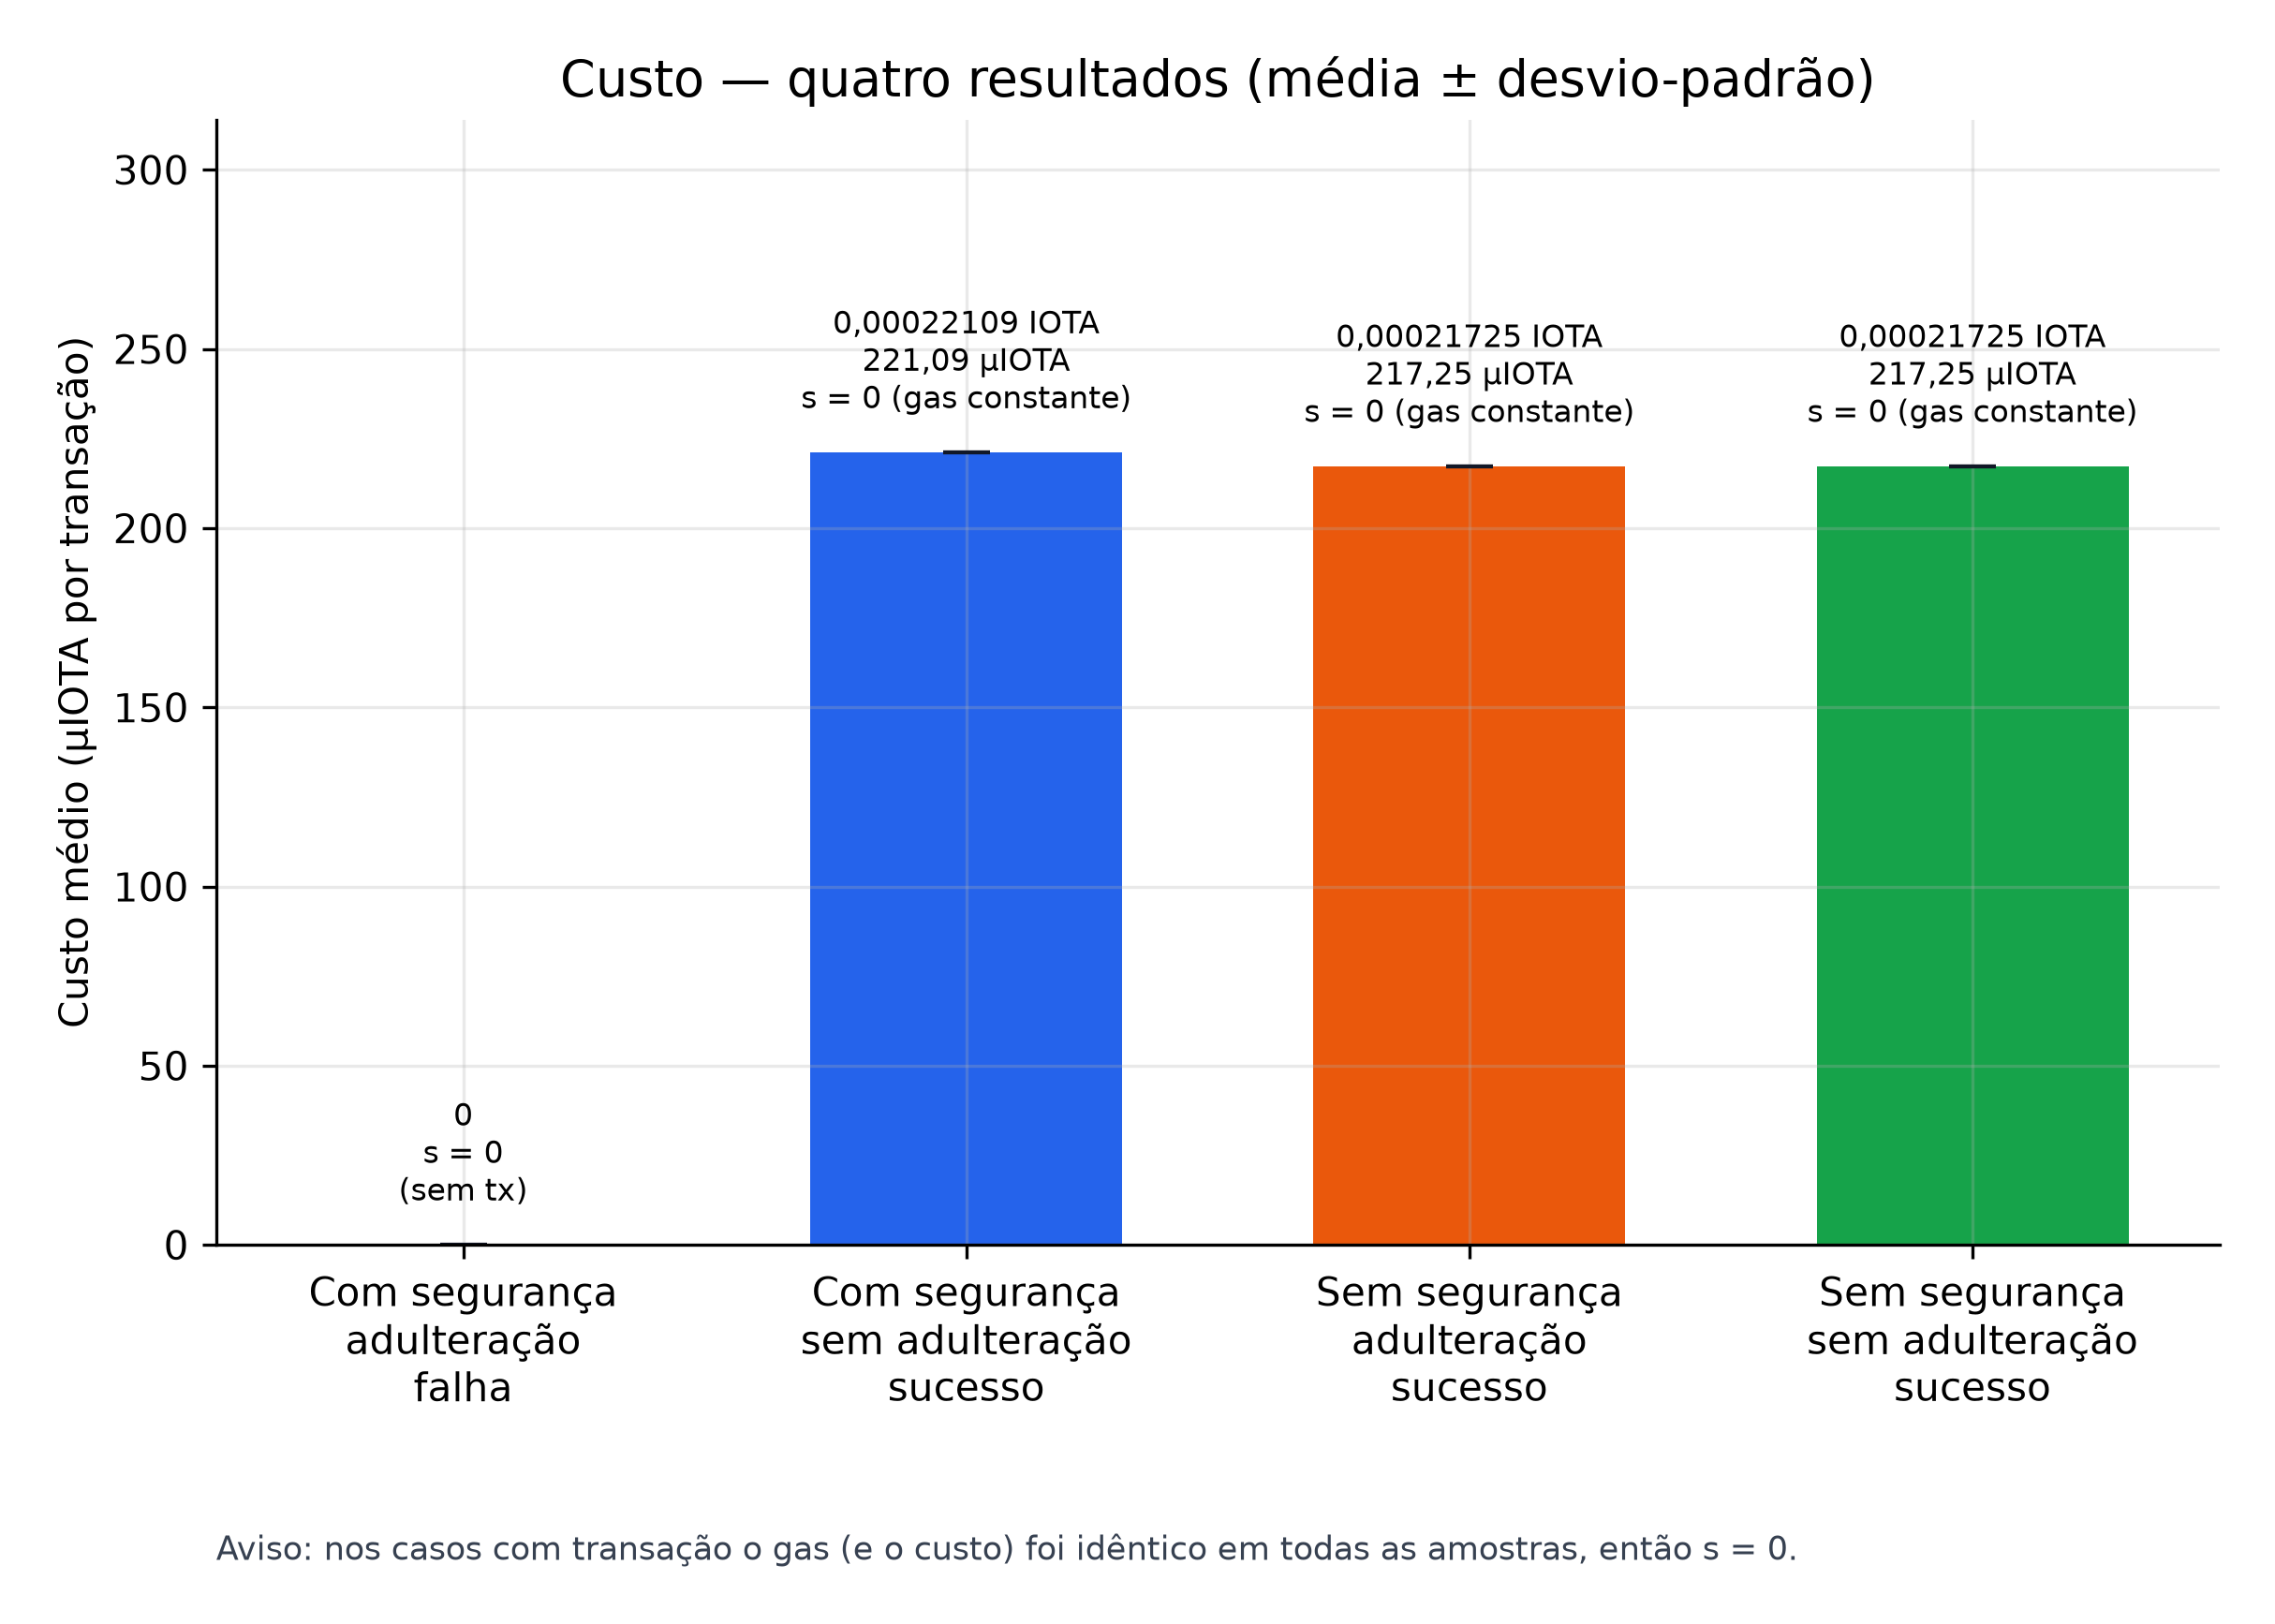
\includegraphics[width=0.92\textwidth]{figuras/custo.png}
\caption{Custo médio por transação nos quatro tratamentos. Nos caminhos que gravaram na cadeia o gás (e o custo) foi constante ($s=0$); com segurança e firmware adulterado não há transação.}
\label{fig:custo}
\end{figure}

O tempo, ao contrário, \emph{tem} desvio-padrão e é dominado pela confirmação do bloco, não pelo filtro de hash (Figura~\ref{fig:tempo}). O overhead de atestação no envio é pequeno --- e, neste lote, o Caso~1 não é mais lento no POST do que o Caso~3. A confirmação mais alta do Caso~1 permanece na faixa de alguns segundos da testnet e não deve ser lida como custo computacional da allowlist. Não há série de tempo de assinatura no ESP32: o chip envia HTTP; a chave EVM assina no computador do relay. Tampouco o lote mede taxa de sucesso \emph{sob carga}: o intervalo entre POSTs foi sequencial.

\begin{figure}[htbp]
\centering
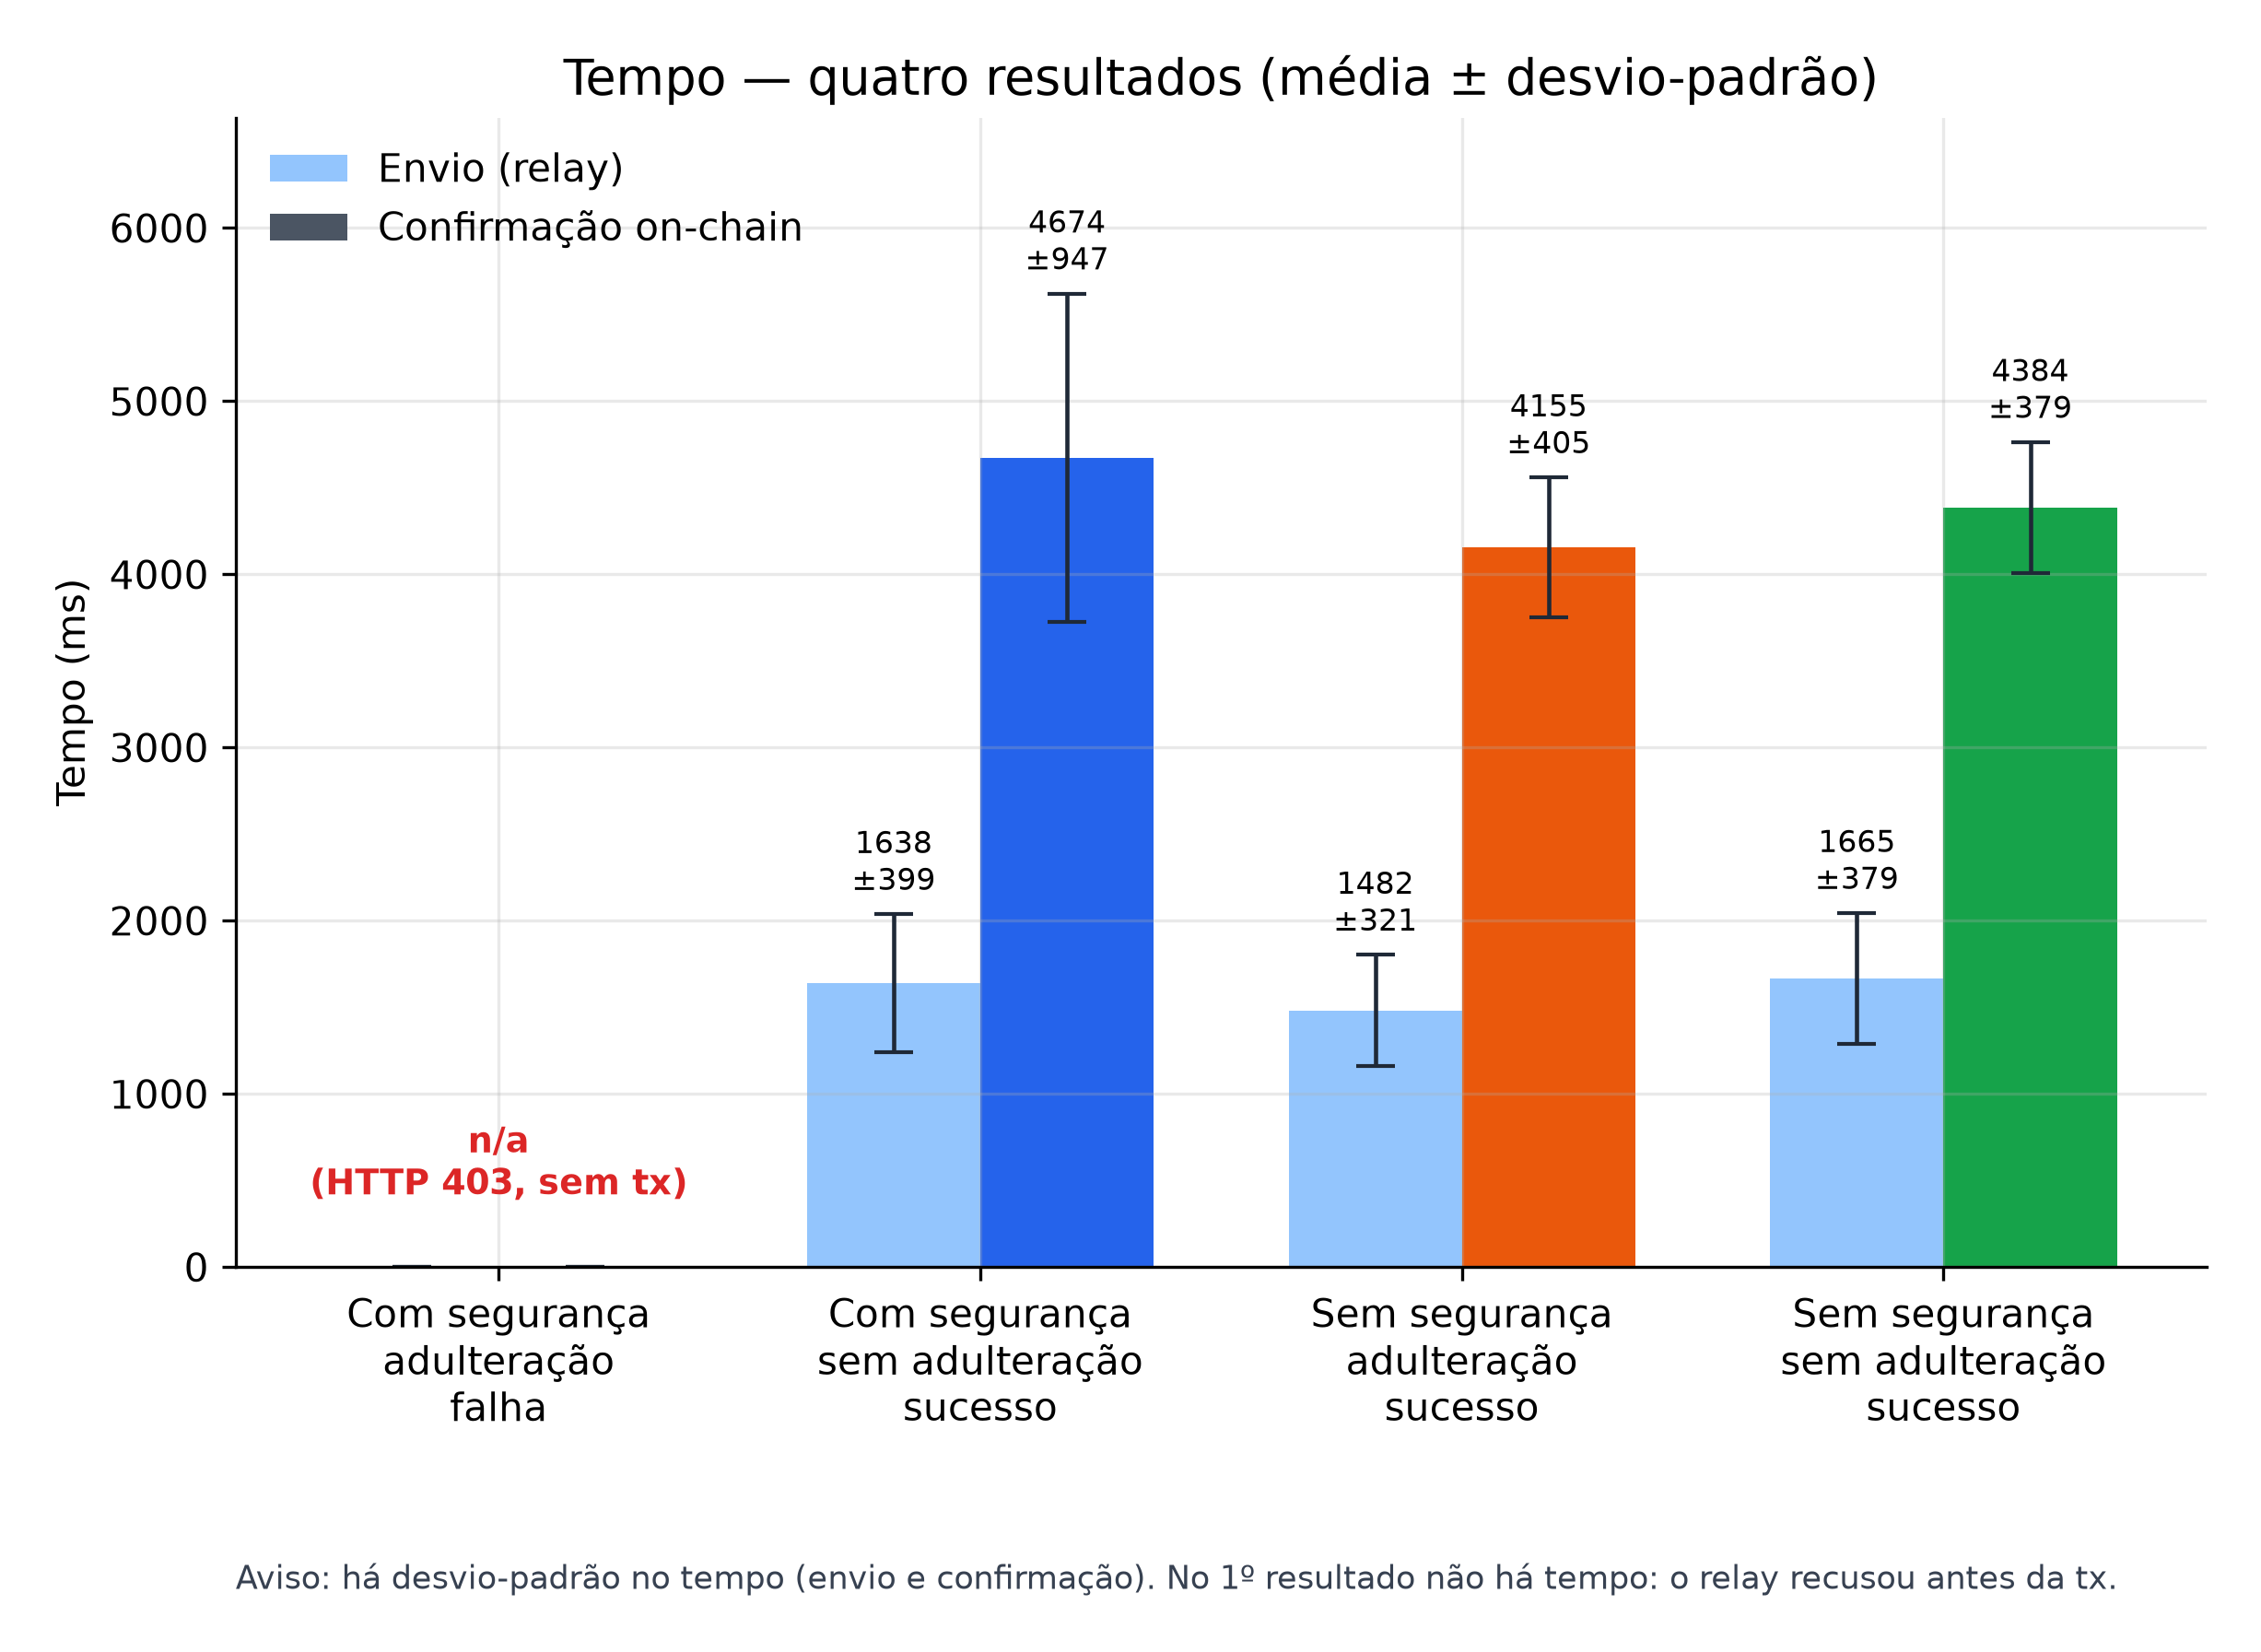
\includegraphics[width=0.92\textwidth]{figuras/tempo.png}
\caption{Tempo médio de envio no relay e de confirmação on-chain (média $\pm$ desvio-padrão). Com segurança e firmware adulterado o tempo é indefinido: o relay responde HTTP 403 antes da transação.}
\label{fig:tempo}
\end{figure}

Esses resultados delimitam o que o experimento \emph{pode} afirmar. A atestação observada é de \emph{arquivo-fonte} (\texttt{.ino}), não da imagem na flash; a identidade on-chain é a da carteira do PC, não de um elemento seguro no dispositivo; o contrato acredita no \texttt{msg.sender} e no payload que o relay monta. Dentro desse perímetro, a conclusão é estreita e útil: a allowlist no intermediário é condição necessária para que firmware adulterado não entre na cadeia; a blockchain, sozinha, não substitui essa verificação. Sem ela, leitura íntegra e leitura adulterada são o mesmo objeto econômico e temporal na testnet.
